\section{Optimizations}

\subsection{Incremental Inference of Convolution and Pooling Layers}\label{sec:ivm}

As explained earlier, occlusion experiments are performed by performing CNN inference on large amounts of images which are generated by masking a small square region of the input image.
When we compare the original image and a single masked image most of the pixel values are not changed. For example for an input image of size $224\times224$ pixels when using a occlusion patch of size $16\times16$ only $0.5\%$ of the pixels are different between the two images.
As a result of this performing a full convolution inference on the masked image introduces lot of redundant computations which could potentially be saved.
For example consider the simple 2D convolution example shown in Figure. \ref{fig:perturbation}.
The input feature map is square map with size $W_1=4$ and is convolved by a 2D square filter kernel of size $F=3$ with a stride of $S=1$ to produce an output feature map of size $W_2=4$.
The input feature map is also padded with zeros with a pad width of $P=1$ to ensure that both the input feature map size and the output feature map size is the same (this step is optional).
Now if we update the top left corner value in the input feature map (marked in red), it will only update 4 output values at the top left corner of the output feature map which corresponds to filter map positions on the input feature map with some overlapping with the updated input value.
Even though in this example the amount of updated values in the output feature maps is $25\%$ of the total output values, in general with larger feature map sizes the portion of updated values will be much smaller.
This analysis similarly applies to pooling layers.

\begin{figure}
  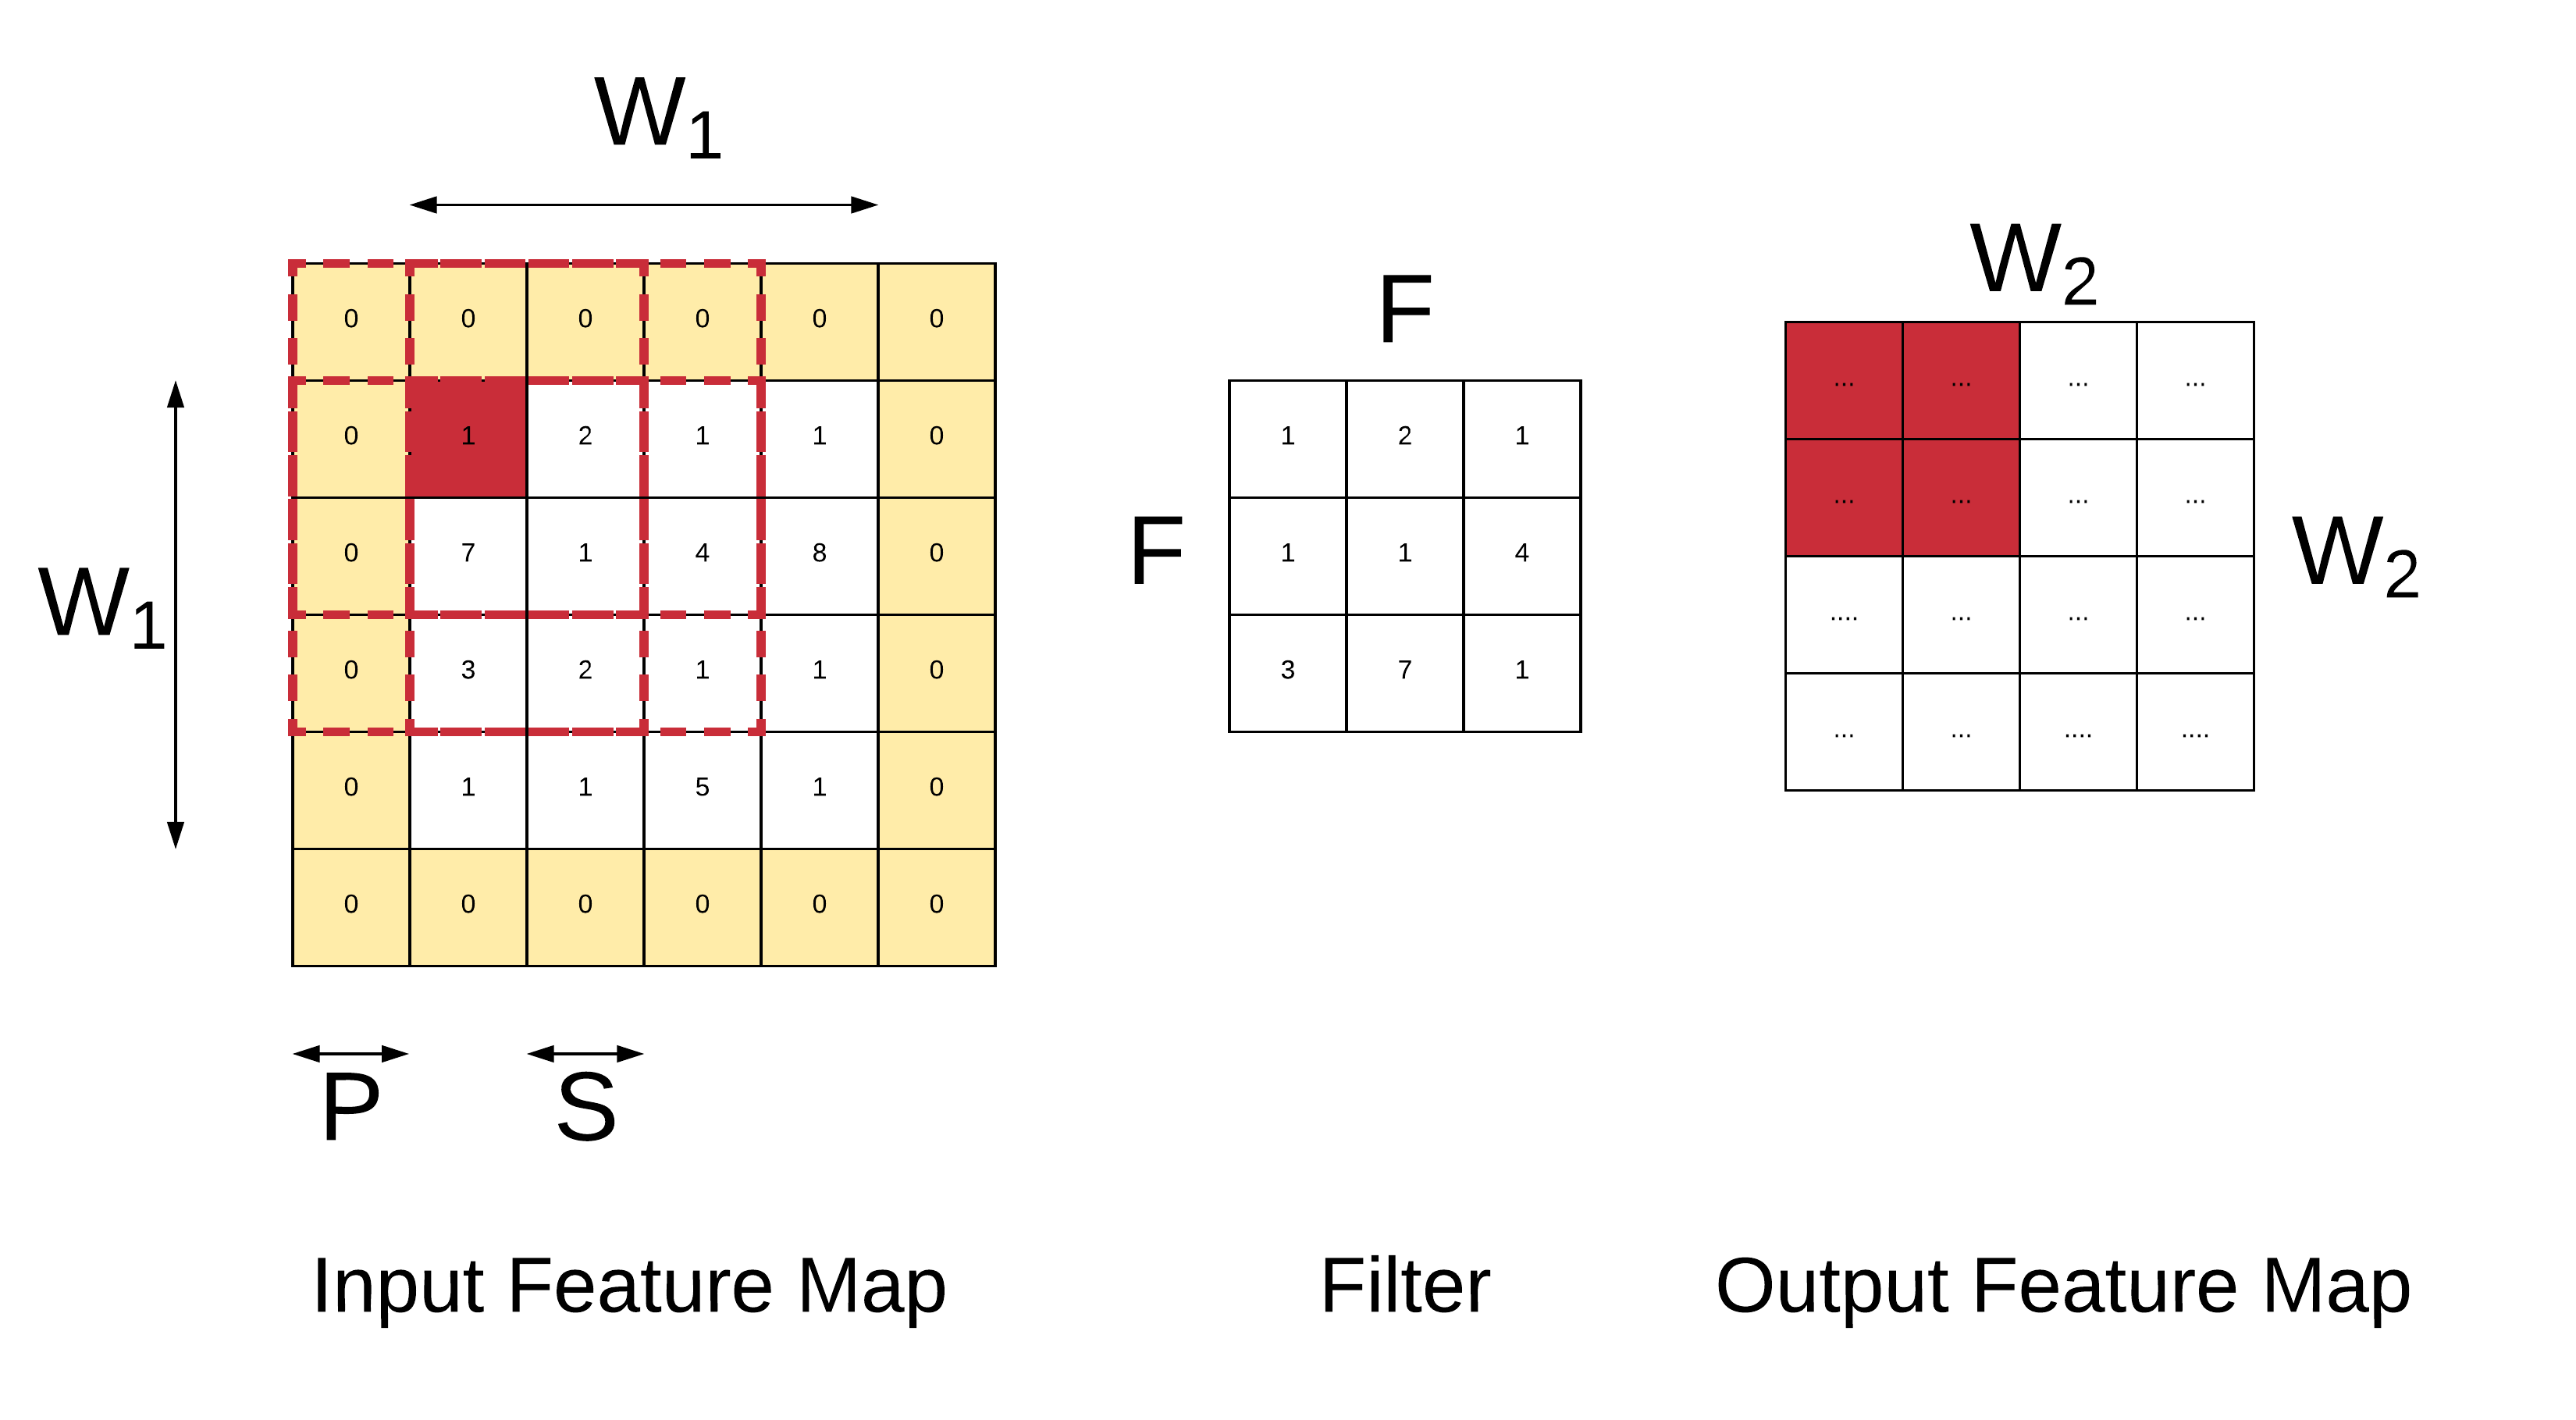
\includegraphics[width=\columnwidth]{./images/small_perturbations}
  \caption{Small perturbations in the input feature map only affect small regions in the output feature map after convolution}
  \label{fig:perturbation}
\end{figure}

More generally the propagation changes in the output feature map of a convolution or pooling layer caused by updating a patch in the input feature map is determined by the filter size $F$ and the stride $S$ of the Conv filter.
For example consider the situation shown in Figure. \ref{fig:patch_propagation}.
Assume a modified patch is placed on the input feature map which spans across $x_{in\_0}\rightarrow x_{in\_1}$ in $x$ dimension and $y_{in\_0}\rightarrow y_{in\_1}$ in y dimension.
Then the coordinates of the modified patch in the output feature map,  $x_{out\_0}\rightarrow x_{out\_1}$ in $x$ dimension and $y_{out\_0}\rightarrow y_{out\_1}$ in y dimension, can be expressed as a function of filter size $F$ and stride $S$ of the Conv/Pool filter as follows:

\begin{figure}
  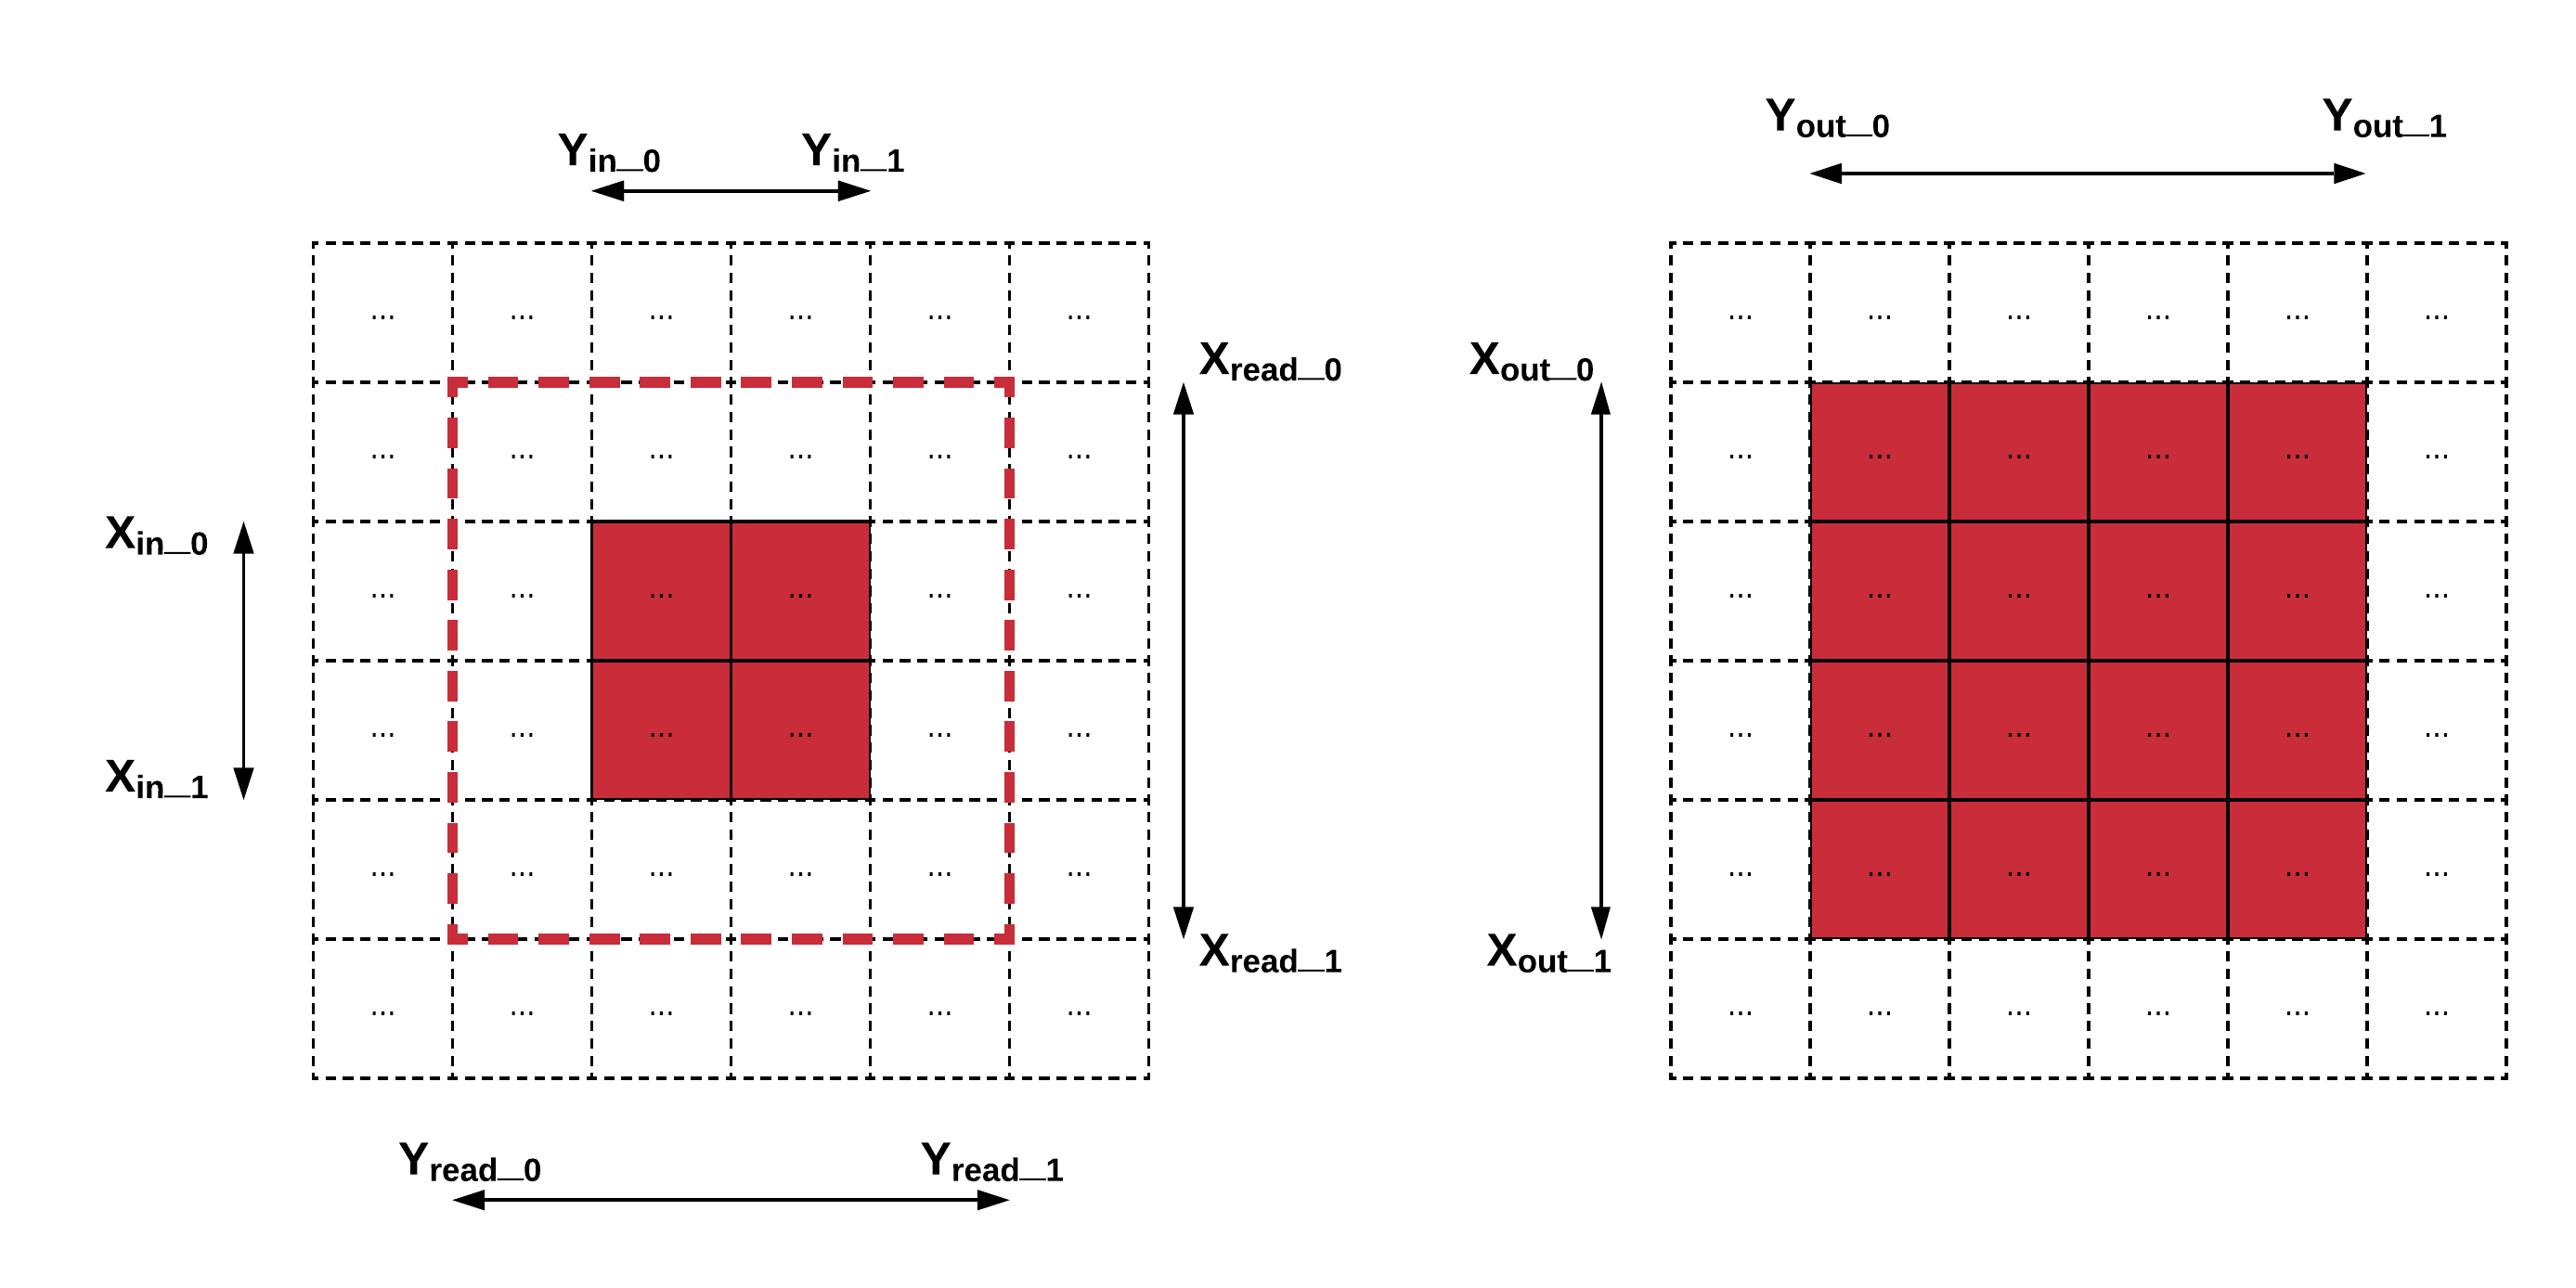
\includegraphics[width=\columnwidth]{./images/patch_propagation}
  \caption{Occlusion patch propagation in Conv layers}
  \label{fig:patch_propagation}
\end{figure}

\begin{equation}
x_{out\_0} = \texttt{max}(\texttt{ceil}((x_{in\_0} - F + 1)/S), 0) \\
\end{equation}
\begin{equation}
x_{out\_1} = \texttt{min}(\texttt{floor}((x_{in\_1} - 1)/S) + 1, W_2) \\
\end{equation}
\begin{equation}
y_{out\_0} = \texttt{max}(\texttt{ceil}((y_{in\_0} - F + 1)/S), 0) \\
\end{equation}
\begin{equation}
y_{out\_1} = \texttt{min}(\texttt{floor}((y_{in\_1} - 1)/S) + 1, W_2)\\
\end{equation}

\vspace{0.2in}

Also not that to compute these values in the output feature map we need to read a slightly bigger region from the input feature map due to the overlapping with the filter positions (marked in red dashed lines in Figure. \ref{fig:patch_propagation}). The coordinates of this read input patch, $x_{read\_0}\rightarrow x_{read\_1}$ in $x$ dimension and $y_{read\_0}\rightarrow y_{read\_1}$ in y dimension, is also a function filter size $F$ and stride $S$ of the Conv filter and can be expressed as follows:

\begin{equation}
x_{read\_0} = \texttt{max}(\texttt{ceil}((x_{in\_0} - F + 1)/S) \times S, 0) \\
\end{equation}
\begin{equation}
x_{read\_1} = \texttt{min}(\texttt{floor}((x_{in\_1} - 1)/S) \times S + F, W_1)\\
\end{equation}
\begin{equation}
y_{read\_0} = \texttt{max}(\texttt{ceil}((y_{in\_0} - F + 1)/S) \times S, 0) \\
\end{equation}
\begin{equation}
y_{read\_1} = \texttt{min}(\texttt{floor}((y_{in\_1} - 1)/S) \times S + F, W_2)\\
\end{equation}

\vspace{0.2in}

\begin{table}[t]
  \centering
  \caption{Notation used in Section. \ref{sec:ivm}}
  \scalebox{0.8}{\begin{tabular}{p{1cm}p{8.5cm}}
    \toprule
    \textbf{Symbol} & \textbf{Description}\\
    \midrule \midrule
    $W_1$ & Width of the input feature map to the Conv/Pool operator\\
    \midrule
    $D_1$ & Depth of the input feature map to the Conv operator\\
    \midrule
    $F$ & Width of filter kernel of the Conv/Pool operator\\
    \midrule
    $W_2$ & Width of the output feature map produced by the Conv/Pool operator\\
    \midrule
    $D_2$ & Depth of the output feature map produced by the Conv operator\\
    \midrule
    $x_{in\_0}$ & Starting x coordinate of the updated patch in the input feature map\\
    \midrule
    $x_{in\_1}$ & Ending x coordinate of the updated patch in the input feature map\\
    \midrule
    $y_{in\_0}$ & Starting y coordinate of the updated patch in the input feature map\\
    \midrule
    $y_{in\_1}$ & Ending y coordinate of the updated patch in the input feature map\\
    \midrule
    $x_{out\_0}$ & Starting x coordinate of the updated patch in the output feature map\\
    \midrule
    $x_{out\_1}$ & Ending x coordinate of the updated patch in the output feature map\\
    \midrule
    $y_{out\_0}$ & Starting y coordinate of the updated patch in the output feature map\\
    \midrule
    $y_{out\_1}$ & Ending y coordinate of the updated patch in the output feature map\\
    \midrule
    $x_{read\_0}$ & Starting x coordinate of the input feature map that need to be used for computing the updated output\\
    \midrule
    $x_{read\_1}$ & Ending x coordinate of the input feature map that need to be used for computing the updated output\\
    \midrule
    $y_{read\_0}$ & Starting y coordinate of the input feature map that need to be used for computing the updated output\\
    \midrule
    $y_{read\_1}$ & Ending y coordinate of the input feature map that need to be used for computing the updated output\\
    \bottomrule
  \end{tabular}}
\label{table:algo_symbols}
\vspace{-2mm}
\end{table}

\subsubsection{Estimating the maximum attainable theoretical speedup}

Important thing to notice with incremental inference of Conv and Pool layers for occlusion experiments is that the size of the updated patch in the output layer is larger than the updated patch in the input layer.
The growth is determined by the filter size and stride. Higher the filter size and stride higher the propagation rate of the modified patch.
With this observation, it is interesting to find out what percentage of computations can be saved by performing incremental inference of Conv and Pooling layers.
This can be easily estimated by iteratively calculating the updated patch sizes for Conv and Pooling layers based on the starting occlusion patch size $W_{patch}$ on the input image for all possible patch locations based on stride used $S_{patch}$.
Algorithm \ref{alg:max-speedup} shows how this can be calculated programmatically.
For sake of simplicity this algorithm assumes that the CNN architecture is a simple chained style architecture instead of more general style of directed-acyclic-graph (DAG).
However the algorithm can be easily extended support more general DAG style architectures.
It takes an object $CNN$ which is a nested information object containing information about different layers of the CNN and their properties, the size of the occlusion patch and the size of the stride for occlusion patch.
It then calculates the floating point operations required for incremental inference versus full inference for each possible location of the occlusion patch and computes the theoretical speedup which is the ratio between operation required for full inference and incremental inference.
It also computes the overall speedup which is the aggregation for all possible positions of the occlusion map and return this value along with 2D array containing individual position wise speedups as the output.

\begin{algorithm}
\caption{Estimate Maximum Theoretical Speedup}\label{alg:max-speedup}
\begin{algorithmic}[1]
\Procedure{EstimateMaxSpeedup}{$CNN$, $W_{patch}$, $S_{patch}$}
\State $flops_{inc} \gets 0$
\State $flops_{full} \gets 0$
\State $tmp \gets floor((CNN.image.W-W_{patch}+1)/S_{patch})$
\State $speedup \gets ARRAY[tmp][tmp]$

\For{\texttt{i in range(0, tmp, $S_{patch}$)}}
  \For{\texttt{i in range(0, tmp, $S_{patch}$)}}
      \State $tmp\_flops_{full} \gets 0$
      \State $tmp\_flops_{inc} \gets 0$
      
      \State $x_{in\_0} \gets i$
      \State $x_{in\_0} \gets i + W_{patch}$
      \State $y_{in\_0} \gets j$
      \State $y_{in\_0} \gets j + W_{patch}$

      \For{\texttt{k in range(0, size(CNN.layers), 1)}}
          \State $layer \gets CNN.layers[k]$
          \If {$layer.type$ $in$ $[conv, pool]$}
            \State $F \gets layer.filter.F$
            \State $S \gets layer.filter.S$
            
            \State $x_{out\_0} = \texttt{max}(\texttt{ceil}((x_{in\_0} - F + 1)/S), 0)$
            \State $x_{out\_1} = \texttt{min}(\texttt{floor}((x_{in\_1} - 1)/S) + 1, W_2)$
            \State $y_{out\_0} = \texttt{max}(\texttt{ceil}((y_{in\_0} - F + 1)/S), 0)$
            \State $y_{out\_1} = \texttt{min}(\texttt{floor}((y_{in\_1} - 1)/S) + 1, W_2)$

            \If {$layer.type$ $=$ $conv$}
              \State $W_1 \gets layer.input.W$
              \State $D_1 \gets layer.input.D$
              \State $W_2 \gets layer.output.W$
              \State $D_2 \gets layer.output.D$

              \State $tmp\_flops_{full} \mathrel{{+}{=}} F^2 \times D_1\times W_2^2\times D_2$
              \State $tmp\_flops_{inc} \mathrel{{+}{=}} F^2 \times D_1$
              \State $\hspace{10mm} \times ~(x_{out\_1} - x_{out\_0})$
              \State $\hspace{10mm} \times ~(y_{out\_1} - y_{out\_0})$
              \State $\hspace{10mm} \times ~D_2$
            \EndIf

            \State $(x_{in\_0}, x_{in\_1}, y_{in\_0}, y_{in\_1})$
            \State $\hspace{10mm} \gets (x_{out\_0}, x_{out\_1}, y_{out\_0}, y_{out\_1})$
          \ElsIf {$layer.type$ $=$ $fully-connected$}
            \State $W_1 \gets layer.input.W$
            \State $W_2 \gets layer.outputs.W$
            \State $tmp\_flops_{full} \mathrel{{+}{=}} W_1 \times W_2$
            \State $tmp\_flops_{inc} \mathrel{{+}{=}} W_1 \times W_2$
          \EndIf
      \EndFor

      \State $flops_{inc} \mathrel{{+}{=}} tmp\_flops_{inc}$
      \State $flops_{full} \mathrel{{+}{=}} tmp\_flops_{full}$
      \State $speedup[i][j] \gets tmp\_flops_{full}/tmp\_flops_{inc}$
      
  \EndFor
\EndFor

\State \textbf{return} ($flops_{full}$/$flops_{inc}$, $speedup$)
\EndProcedure
\end{algorithmic}
\end{algorithm}

We have applied this algorithm to analyze the theoretical maximum attainable speedup for many widely used CNN architectures by performing static analyzing on the CNN models defined using PyTorch framework (see Figure. \ref{fig:speedups}).
With an occlusion patch of size 16, moved with a stride of 1, for most CNN architectures we can achieve an average speedup of around 2.
However VGG and Squeezenet1\_0 CNN architectures can produce higher speedups than this.
The reason for this is VGG (16 and 19 layer versions) and Squeezenet1\_0 architectures use smaller Conv filter kernels $(3\times3)$. Therefore the rate of propagation of the occlusion patch is slower than other CNN architectures.
Thus more redundant computations can be saved from those architectures by applying incremental inference approach.

\begin{figure}
  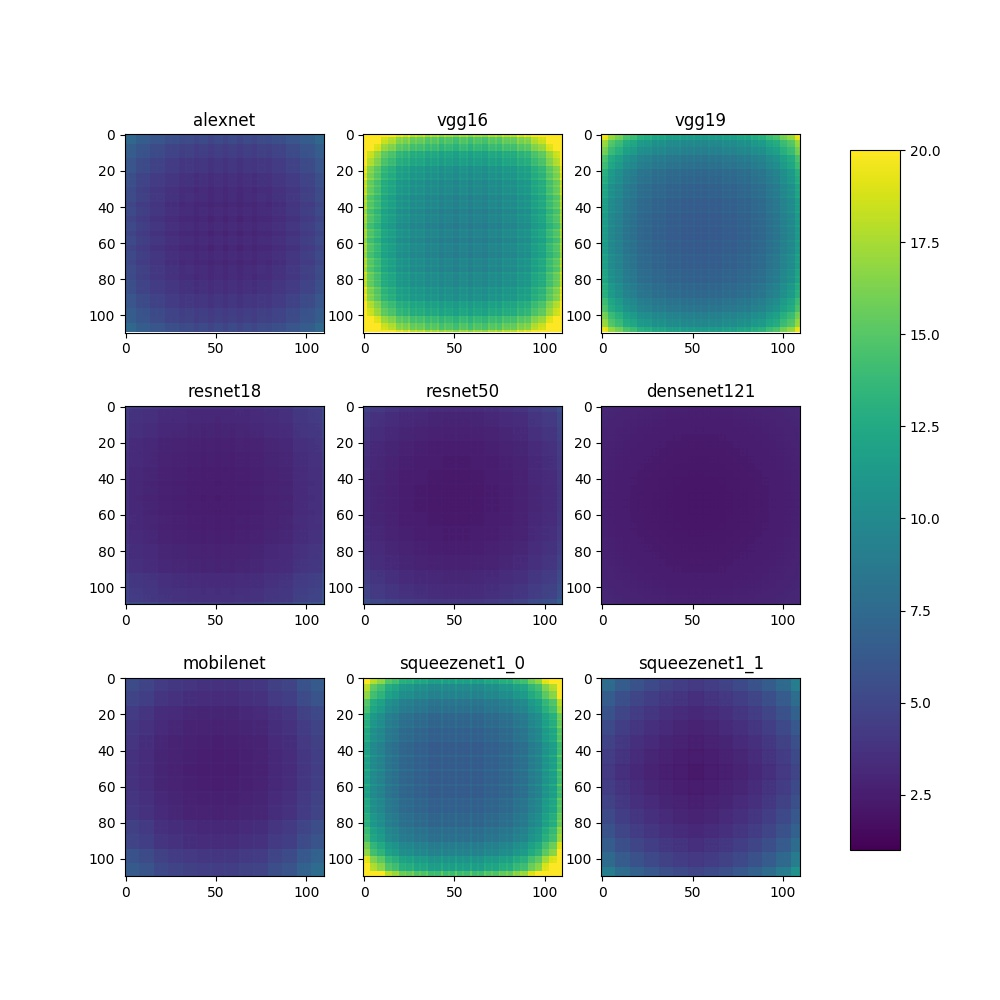
\includegraphics[width=\columnwidth]{./images/speedup_plots}
  \caption{Maximum attainable theoretical speedup for incremental inference approach for an occlusion experiment with patch of size 16 pixels stride of 2}
  \label{fig:speedups}
\end{figure}

\subsubsection{Occlusion Experiment with Incremental Inference}
With all the necessary core ideas explained, we now explain how incremental inference approach can be used to implement occlusion experiment (see Algorithm. \ref{alg:inc-inference}).
On a high-level the structure of this algorithm is similar to the theoretical speedup calculation algorithm. But the following differences can be noted. The algorithm takes an input image $I$ as input for the occlusion experiment in addition to the CNN model, patch width $W_{patch}$, and stride $S_{patch}$.
It then performs a full inference on the image and obtain a list containing activations for all the layers, including input image, by calling the method \texttt{PerformFullCNNInference(CNN, I)}.
It then finds the index of the predicted class label by finding the index of the maximum activation in the softmax layer, which is the last layer in the CNN.
Next similar to Algorithm. \ref{alg:max-speedup}, it iterates through all the possible positions of the occlusion patch on the input image and perform incremental inference for Conv and Pool layers based on the updated patch locations. For fully-connected and softmax layers usual full-inference is performed as there is no redundancy in computations.
When performing incremental inference for Conv and Pooling layers, the updated output of the previous layers is stitched together with pre-materialized values obtained from full inference ($M$) corresponding to that layer to create the input patch for the incremental inference operator.

Similar to speedup calculations, for simplicity, the algorithm here assumes the CNN architecture is a simple chain styled architecture. However it can be easily extended to support more general DAG style CNN architectures.
Another point to notice is that this algorithm performs inference for single occlusion position at a time. Alternatively one could batch together multiple occlusion patch positions together and perform batched inference. However since the patch sizes are not guaranteed to be the same at each layer, they may be need to be padded to transform them into the same size.
Batching multiple inferences together can reduce the runtime of occlusion experiments as it can amortize the overheads specially when using GPUs for inference.

\begin{algorithm}
\caption{Occlusion Experiment with Incremental Inference}\label{alg:inc-inference}
\begin{algorithmic}[1]
\Procedure{OcclusionWithIncrementalInference}{$I$,$CNN$, $W_{patch}$, $S_{patch}$}

\State $M \gets \texttt{PerformFullCNNInference}(CNN, I)$
\State $label_{index} \gets argmax(M[-1])$
\State $tmp \gets floor((CNN.image.W-W_{patch}+1)/S_{patch})$
\State $P \gets ARRAY[tmp][tmp]$

\For{\texttt{i in range(0, tmp, $S_{patch}$)}}
  \For{\texttt{i in range(0, tmp, $S_{patch}$)}}

      \State $x_{in\_0} \gets i$
      \State $x_{in\_0} \gets i + W_{patch}$
      \State $y_{in\_0} \gets j$
      \State $y_{in\_0} \gets j + W_{patch}$

      \State $x \gets Zero[x_{in\_1}-x_{in\_0}][y_{in\_1}][y_{in\_0}]$
      
      \For{\texttt{k in range(0, size(CNN.layers), 1)}}
          \State $layer \gets CNN.layers[k]$
          \If {$layer.type$ $in$ $[conv, pool]$}

            \State $x_{read\_0} \gets \texttt{max}(\texttt{ceil}((x_{in\_0} - F + 1)/S)$
            \State $\hspace{10mm} \times ~S, 0)$
            \State $x_{read\_1} \gets \texttt{min}(\texttt{floor}((x_{in\_1} - 1)/S)$
            \State $\hspace{10mm} \times ~S + F, W_1)$
            \State $y_{read\_0} \gets \texttt{max}(\texttt{ceil}((y_{in\_0} - F + 1)/S)$
            \State $\hspace{10mm} \times ~S, 0)$
            \State $y_{read\_1} \gets \texttt{min}(\texttt{floor}((y_{in\_1} - 1)/S)$
            \State $\hspace{10mm} \times ~S + F, W_2)$

            \State $tmp \gets M[k]$
            \State $tmp[x_{in\_0}:x_{in\_1}][y_{in\_0}:y_{in\_1}] \gets x$

            \State $x \gets tmp[x_{read\_1}-x_{read\_0}]$
            \State $\hspace{20mm}       [y_{read\_1}-y_{read\_0}]$

            \State $x \gets layer.transform(x)$

            \State $F \gets layer.filter.F$
            \State $S \gets layer.filter.S$
            
            \State $x_{out\_0} = \texttt{max}(\texttt{ceil}((x_{in\_0} - F + 1)/S), 0)$
            \State $x_{out\_1} = \texttt{min}(\texttt{floor}((x_{in\_1} - 1)/S) + 1, W_2)$
            \State $y_{out\_0} = \texttt{max}(\texttt{ceil}((y_{in\_0} - F + 1)/S), 0)$
            \State $y_{out\_1} = \texttt{min}(\texttt{floor}((y_{in\_1} - 1)/S) + 1, W_2)$
            
            \State $(x_{in\_0}, x_{in\_1}, y_{in\_0}, y_{in\_1})$
            \State $\hspace{10mm} \gets (x_{out\_0}, x_{out\_1}, y_{out\_0}, y_{out\_1})$
          \ElsIf {$layer.type$ $=$ $fully-connected$}
            \State $tmp \gets CNN.layers[k-1].type$
            \If {$tmp \mathrel{{!}{=}} fully-connected$}
              \State $tmp \gets M[k-1]$
              \State $tmp[x_{out\_0}:x_{out\_1}]$$[y_{out\_0}:y_{out\_1}]$$\gets x$
              \State $x \gets tmp$
            \EndIf
            \State $x \gets fully-connected(x, layer.weights)$
          \ElsIf {$layer.type$ $=$ $softmax$}
            \State $x \gets softmax(x)$
          \EndIf
      \EndFor

      \State $P[i][j] \gets x[label_{index}]$
      
  \EndFor
\EndFor

\State \textbf{return} $(label_{index}, P)$
\EndProcedure
\end{algorithmic}
\end{algorithm}